\chapter{Teoretický rozbor}
\label{chap:teoreticky-rozbor}
Táto kapitola sa zaoberá teoretickým rozborom problematiky chronických rán, ktoré sú jadrom tejto práce. Kapitola sa snaží najprv vysvetliť základné pojmy a termíny týkajúce sa problematiky a následne vysvetľuje samotné chronické rany, ich príčiny vzniku a prejavy. Celá kapitola vychádza z informácií dostupných na webovej stránke \cite{pcCdSrbbhhlr5YcQ} a z kníh \cite{Hlinkova2015} a \cite{Pokorna2012}.  

%%%%%%%%%%%%%%%%%%%%%%%%%%%%%%%%%%%%%%%%%%%%%%%%%%%%%%%%%%%%%%
\section{Koža}
Koža je najväčší orgán ľudského tela, ktorý má u dospelého človeka veľkosť plochy od 1,6 až do 1,8 metra štvorcového a váži približne 7 percent celkovej telesnej hmotnosti. Hrúbka kože sa pohybuje od 0,4 až po 4 milimetre a líši sa podľa jednotlivých častí tela. Najtenšia je na očných viečkach, najhrubšia zase na chrbte.

Kože nielenže plní funkciu obalu človeka, ale okrem toho plní aj celú radu pre človeka oveľa dôležitejších funkcií, medzi ktoré patrí:
\begin{itemize}  
\item \textbf{ochrana -} pred vstupom nečistôt do organizmu, pred stratou tekutín, proti teplotným výkyvom
\item \textbf{vnímanie -} zmyslové buky v koži informujú o teplote alebo poranení
\item \textbf{termoregulácia -} tepelná izolácia, výmena tepla medzi organizmom a okolím
\item \textbf{skladovanie -} koža sa podiela na látkovej výmene a uchovávaní tukov, vody, minerálnych látok a vitamínov
\item \textbf{vylučovanie -} mazové a potné žľazy vylučujú vodu, soli, tuky, oxid uhličitý a dusíkaté látky.
\item \textbf{vstrebávanie -} kožou prenikajú látky rozpustné v tukoch a dýchacie plyny
\item \textbf{estetická funkcia -} vzhľad a úprava kože je jedným z prvých znakov, ktorých si ľudia pri vzájomnom kontakte všímajú
\end{itemize}

Kôža je zložená z 3 hlavných časti, a to z pokožky (epidermis), zamši (dermis) a podkožia (subcutis). Tieto 3 hlavné vrstvy je možné vidieť na obrázku dole. Okrem týchto hlavných vrstiev sa skladá aj z vlasov/chlpov, nechtov a žliaz (mazové, potné, pachové a mliečne). Dokopy sa nazývajú kožné deriváty. 
\begin{itemize}  
\item \textbf{Pokožka -} vonkajšia vrstva. Je tvorená niekoľkými vrstvami kožných buniek. V spodných častiach pokožky sa bunky neustále delia a vytláčajú bunky nad sebou bližšie k povrchu. Postupom do horných vrstiev pokožky bunky postupne rohovatejú, odumierajú a odlupujú sa. Pomocou tohoto procesu dochádza k plynulej obmene celej pokožky. Z človeka sa počas jeho života odlúpne v priemere asi 20 kilogramov mŕtvych buniek. 
\item \textbf{Zamša -} stredná vrstva. Je tvorená väzivom, sieťou ciev a nervových zakončení. Táto vrstva rozhoduje o pevnosti kože, jej pružnosti a mechanickej odolnosti. Medzi dôležité súčasti zamše patria hlavne nervové zakončenia, vďaka ktorým vnímame teplo, chlad a bolesť. Jemné cievy zase slúžia pre reguláciu tepla a imunitné bunky zaisťujú ochranu.
\item \textbf{Podkožie -} najhlbšia vrstva. Je tvorená riedkym väzivom a tukom. Hlavnou úlohou podkožia je ochrana proti teplotným vplyvom a mechanickému poškodeniu. V tukovom tkanive si organizmus uchováva prebytky energie. 
\end{itemize}
\begin{figure}[h]
  \centering
  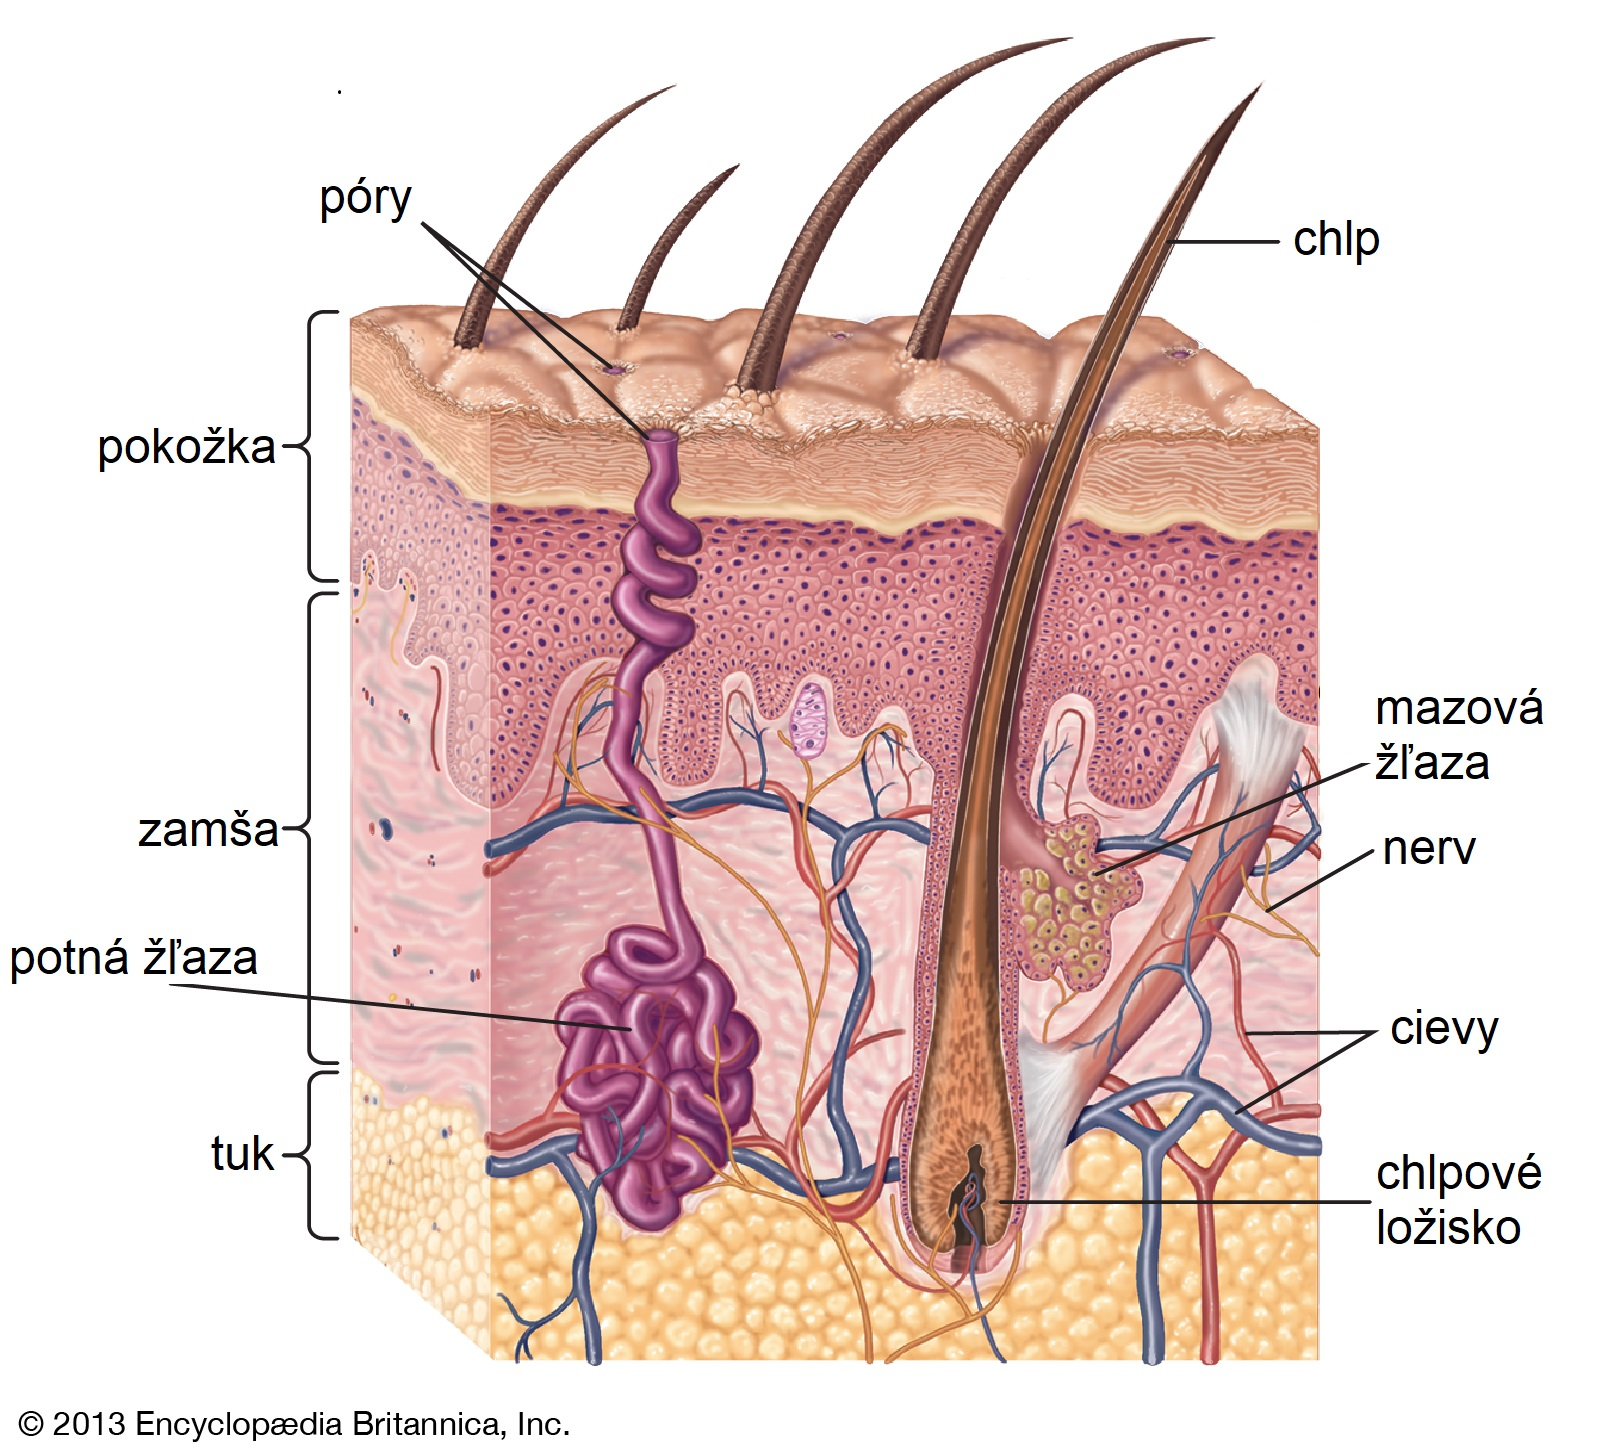
\includegraphics[scale=0.20]{fig/koza.jpg}
  \caption{Zloženie ľudskej kože. Zdroj \cite{Ebling2016}}
  \label{fig:koza}
\end{figure}

%%%%%%%%%%%%%%%%%%%%%%%%%%%%%%%%%%%%%%%%%%%%%%%%%%%%%%%%%%%%%%
\section{Kožná rana}
Kožná rana je definovaná ako strata, či prerušenie kožného krytu v dôsledku fyzikálneho, mechanického, alebo termického poškodenia, či v dôsledku patofyziologických porúch, alebo akékoľvek poškodenie anatomických, alebo fyziologických funkcií tkaniva.

Kožné rany je možné rozdeliť na jednoduché a komplikované. Jednoduché kožné rany zasahujú do pokožky, zamše a podkožného tuku. Komplikované rany zase narozdiel od jednoduchých prenikajú hlbšie a poškodzujú dôležité nervovo-cievne zväzky a orgány. Komplikované rany je ďalej možné rozdeliť na penetrujúce a nepenetrujúce. Penetrujúca rana preniká do teľnej dutiny. Nepenetrujúca rana naopak nepreniká do telesnej dutiny. U každej rany, či už jednoduchej, komplikovanej, penetrujúcej, alebo nepenetrujúcej určujeme a popisujeme vlastnosti, ktoré sú veľmi dôležité pri sledovaní procesu hojenia rany a voľby optimálnej liečby. Medzi takéto vlastnosti patrí:
\begin{itemize} 
\item lokalizácia rany
\item veľkosť rany
\item hĺbka rany
\item tvar rany
\item smer rany
\item okraje rany
\end{itemize}

%%%%%%%%%%%%%%%%%%%%%%%%%%%%%%%%%%%%%%%%%%%%%%%%%%%%%%%%%%%%%%
\section{Triedenie a typy rán}
Rany a poškodenia je možné deliť do niekoľko skupín podľa rôznych kritérií. Rany sa delia podľa ich priebehu, podľa rozsahu ich poškodenia, podľa množstva choroboplodných zárodkov, podľa spôsobu hojenia, podľa lokalizácie, podľa postihnutých štruktúr a mnoho iných delení, pričom najdôležitejšie delenia sú tie, ktoré sú ďalej popísané podrobnejšie.
Rany podľa priebehu sa delia na:
\begin{itemize} 
\item \textbf{akútne rany -} vznikajú v zdravom kožnom tkanive. Hoja sa obvykle v krátkom čase a bez komplikácií.
\item \textbf{chronické rany -} trvajú dlhšie než 4 týždne, alebo to sú rany, ktoré vznikajú v zmenenom tkanive, a ktoré aj cez všetku odpovedajúcu liečbu nevykazujú známky hojenia.
\end{itemize}
Rany podľa rozsahu sa delia na:
\begin{itemize} 
\item \textbf{uzatvorené rany -} poškodenie bez porušenia integrity kože
\item \textbf{povrchové rany -} poškodenia pokožky
\item \textbf{hlboké rany -} poškodenie až do podkožia
\item \textbf{prenikajúce rany -} zasahujú do teľných dutín
\item \textbf{komplikované rany -} komplexné rozsiahle poranenia s možným poškodením ciev, nervov, svalov, kostí a orgánov
\end{itemize}
Rany podľa množstva choroboplodných zárodkov sa delia na:
\begin{itemize} 
\item \textbf{aseptické rany -} bez zárodkov (chirurgický rez)
\item \textbf{kontaminované rany -} s prítomnosťou zárodkov, ktoré však nemusia vyvolať infekciu
\item \textbf{infikované rany -} s premnoženými mikroorgnizmami (rany vzniknuté po pohryznutí, poprípade zanedbané, alebo zastaralé rany)
\end{itemize}
Rany podľa spôsobu hojenia sa delia na:
\begin{itemize} 
\item \textbf{rany s primárnym hojením -} vďaka zlepeniu/zošitiu okrajov rany nevzniká nové spojivové tkanivo
\item \textbf{rany so sekundárnym hojením -} rana sa hojí novo tvoreným tkanivom
\end{itemize}

%%%%%%%%%%%%%%%%%%%%%%%%%%%%%%%%%%%%%%%%%%%%%%%%%%%%%%%%%%%%%%
\section{Príčiny rán}
Rany môžu vznikať pôsobením rôznych príčin, medzi ktoré patria vonkajšie, vnútorné príčiny alebo kombinácia týchto dvoch. Medzi vonkajšie príčiny patria rany rezné, sečné, tržné, rany spôsobené pohryznutím, bodné, strelné, zhmoždené, popáleniny, omrzliny, poleptaniny a rany spôsobené z ožiarenia. Medzi vnútorné príčiny patria cievne vredy dolných končatín, neuropatické vredy, preležaniny, rany pri nádorových ochoreniach, rany pri infekčných ochoreniach a rany pri imunitných poruchách. Vo všeobecnosti sa dajú príčiny vzniku rán rozdeliť do troch základných oblastí a to podľa toho, na akom základe vznikajú:
\begin{itemize} 
\item lokálne poruchy výživy kože
\item lokálneho pôsobenia tlaku, cievneho poškodenia
\item systémového ochorenia (infekčného, nádorového, krvného...)
\end{itemize}

%%%%%%%%%%%%%%%%%%%%%%%%%%%%%%%%%%%%%%%%%%%%%%%%%%%%%%%%%%%%%%
\section{Chronické rany}
V kapitole Triedenie a typy rán boli rany rozdelené podľa priebehu na akútne a chronické. 

Akútne rany nie sú predmetom tejto práce, avšak pre celistvosť sú tu uvedené. Akútna rana je porušenie integrity tkaniva teľa vzniknuté v dôsledku fyzikálneho, mechanického, alebo termického poškodenia. Vznikajú v zdravom kožnom tkanive. Hoja sa obvykle v krátkom čase a bez komplikácií. Ich príčinou je väčšinou úraz, alebo chirurgický zákrok. Patria sem rany mechanické, traumatické, termické, chemické, aktinické, opary a pľuzgiere.

Chronická rana je sekundárne hojaca sa rana, ktorá aj napriek adekvátnej liečbe nemá po dobu 4 týždňov tendenciu sa uzdravovať. Chronické rany sa hoja výstavbou nového tkaniva. Doba hojenia je preto spravidla dlhá a závisí na príčine a rozsahu poškodeného tkaniva. Chronické rany môžu vzniknúť aj z akútnych rán a to tak, že akútna rana je neadekvátne ošetrená, prípadne vznikne infekcia. Chronické rany sa taktiež objavujú v patologicky zmenených tkanivách a za príčinu ich vzniku sa najčastejšie označuje lokálne poruchy výživy kože, pôsobenie tlaku, poškodenie cievneho systému, alebo systémové ochorenie. Medzi najčastejšie chronické rany patria bercové vredy, dekubity (preležaniny), diabetická noha, nádory s vredovým rozpadom, alebo komplikovane sa hojace pooperačné rany.

\subsection{Bercové vredy}
Bercové vredy sú poškodením kožného krytu zasahujúce rôzne hlboko do podkožného tkaniva v oblasti členku. Nachádza sa najčastejšie v miestach medzi kolenom a členkom, hlavne v oblasti vnútorného členku.

Príčinou vzniku vredov býva drobné poranenie, alebo infekcia. Väčšina bercových vredov je žilného pôvodu a sú prejavom hromadenia krvi v dolných končatinách. Pri pretlaku v žilnom riečisku dochádza k žilnej nedostatočnosti. Žily na končatinách sa rozširujú, chlopne strácajú svoju správnu funkciu a prepúšťajú časť krvi naspäť. Prietok končatinami sa spomaľuje, tekutina z krvi v preplnených žilách prestupuje do podkožia, rozvíja sa opuch, ktorého následkom dochádza k poruche výživy kože. 

Prvým prejavom toho, že vzniká bercov vred je miestne začervenanie. Koža nad postihnutým miestom sa ztenčuje, je suchá, môže ju prekrývať šedivý ekzém a toto miesto je často dobre ohraničené s rovnými okrajmi. Bercove vredy bývajú rozsiahle, vlhké, skôr plytké a s povlečenou spodinou. Väčšinou sú sprevádzané rozsiahlym opuchom postihnutej oblasti a ďalšími kožnými zmenami. Okolie vredu vykazuje známky žilnej nedostatočnosti, hromadenie pigmentu, stráta ochlpenia. Bercové vredy sú často bolestivé.
\begin{figure}[h]
  \centering
  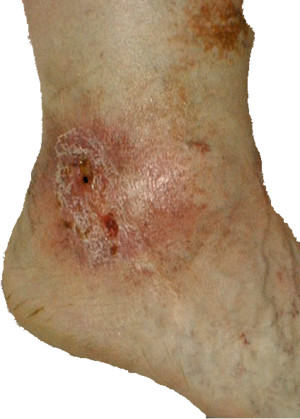
\includegraphics[scale=0.50]{fig/bercov-vred.png}
  \caption{Bercov vred žilného pôvodu. Zdroj \cite{BsyXZC783dJbfdc7}}
  \label{fig:bercov-vred}
\end{figure}

\subsection{Dekubity}
Dekubity, známe tiež ako preležaniny, sú rany spôsobené pôsobením lokálneho tlaku na kožu. Vznikajú v miestach dlhodobého kontaktu kože s podložkou. Sú typické pre chorých ľudí, ktorý sú dlhodobo pripútaný na lôžko.

Príčinou vzniku preleženín je to, že v miestach neustáleho kontaktu a tlaku dochádza k uzatvoreniu drobných ciev. Tkanivo je zle zásobované živinami a kyslíkom, a tak dochádza k ich postupnému odumieraniu. Rozsah odumretia tkaniva závisí na vzájomnom pôsobení niekoľkých faktorov. Konkrétne závisí na intenzite tlaku, doby pôsobenia tlaku, odolnosti organizmu voči tlaku, celkového stavu postihnutia a vplyvov vonkajšieho prostredia. Preležaniny sa objavujú pomerne rýchlo, v ojedinelých prípadoch už po niekoľkých hodinách.

K miestam najnáchylnejším k vzniku dekubitov patria oblasti s malou vrstvou tukového a svalového tkaniva, kde z vonka pôsobí tlak priamo na kosti. Medzi takéto oblasti patrí oblasť nad krížovou kosťou, päty, sedacie kosti, oblasť nad veľkými výčnelkami stehennej kosti a vonkajšie členky. Avšak napriek tomu sa môžu vytvoriť kdekoľvek na tele. Vývoj preležanín prebieha v niekoľkých štádiách. Prvým prejavom je začervenanie, bolestivosť a opuchnutie kože. Nasleduje pľuzgier, alebo povrchový vred zasahujúci do pokožky a zamše, v okolí sa rozvíja zápal. Posledným štádiom je odumretie tkaniva. Nedostatočne liečená preležanina sa ďalej prehlbuje, odumreté tkanivo sa topí, hnilobne páchne a zvyšky tkaniva majú žltozelenú farbu.
\begin{figure}[h]
  \centering
  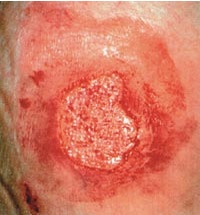
\includegraphics[scale=1]{fig/dekubit.png}
  \caption{Preležanina v druhom štádií. Zdroj \cite{Vilimovsky2015}}
  \label{fig:dekubit}
\end{figure}

\subsection{Diabetická noha}
Syndrómom diabetickej nohy sa označujú defekty dolných končatín, spôsobené postihnutím ciev a nervov. Ide o komplikáciu ochorenia cukrovky.

Medzi 2 hlavné príčiny vzniku tohoto syndrómu sa dá označiť diabetická neuropatia a ischemická choroba dolných končatín. Diabetickou neuropatiou je myslená dlhodobo zvýšená hladina cukru v krvi, ktorá poškodzuje funkciu a štruktúru periférnych nervov. Postihnutie sa týka všetkých typov nervových vlákien. Obmedzenie, alebo strata funkcie ma priamy dopad na nohu:
\begin{itemize}
\item \textbf{senzorická neuropatia -} vedie k strate citlivosti na bolesť, teplotu, vibrácie, tlak a polohocit.
\item \textbf{motorická neuropatia -} vedie k oslabeniu a skráteniu svalstva a vzniku otlakov.
\item \textbf{vegetatívna neuropatia -} vedie k zníženému poteniu kože, strate jej pružnosti a tým k vyššiemu riziku prasklín.
\end{itemize}

Za ischemickú chorobu dolných končatín sa označuje ochorenie tepien, ktoré spôsobuje nedostatočné prekrvenie dolných končatín. Hlavnou príčinou ochorenia je ateroskleróza, ktorá má za následok zúženie, alebo úplný uzáver tepien a obmedzenie prítoku krvi. Okrem veľkých ciev sú v prípade diabetickej nohy postihnuté aj jemné vlásočnice. Takto nedostatočne prekrvené tkanivo je náchylné k poraneniu a vykazuje zlú hojivosť.

Medzi prejavy diabetickej nohy v kľude patria nepríjemné pálčivé bolesti, brnenie, alebo mravenčenie končatín. Pri chôdzi sa zase prejavuje pocitom stiahnutia okolo členkov. Koža nohy je suchá a šúpe sa. Svaly lýtok sú oslabené, ochlpenie je preriedené, alebo chýba úplne. Pri nedokrvení končatín sa môže objaviť aj bolesť, ale nie je to pravidlom. Najčastejším miestom vzniku sú členky, priehlavok, päta a prsty. Medzi ďalšie prejavy patria praskliny, pľuzgiere a odreniny, ktoré keď sa neliečia, tak sa rozširujú, poprípade sa do toho pridá infekcia.
\begin{figure}[h]
  \centering
  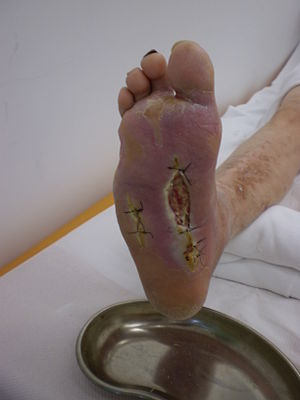
\includegraphics[scale=2]{fig/diabeticka-noha.jpg}
  \caption{Syndróm diabetickej nohy. Zdroj \cite{uGOum7N9LzIGa5X2}}
  \label{fig:diabeticka-noha}
\end{figure}

\subsection{Maligne rany}
Nehojace sa rany a kožné defekty, ktoré vznikajú pri nádorových ochoreniach sa nazývajú maligne rany. Vyskytujú sa najčastejšie u pacientov s pokročilými nádorovými ochoreniami. Vznikajú v súvislosti so spinocelulárnym karcinonom, bazocelulárnym karcinonom, malignym melanonom, alebo zhubným nádorom (pŕs, hlavy, krku,...).

Príčiny vzniku týchto rán sa dajú zhrnúť do 3 oblastí: Primárne kožný nádor, prerastanie nádoru mäkkých tkanív do kože a kožné metastázy nádoru. Rastom nádoru dochádza k narušeniu kožných kapilár a lymfatických ciev a k útlaku okolných tkanív. To vedie k obmedzeniu prísunu živín a vzniku nekrózy.

Na začiatku sa v koži najčastejšie objaví zatvrdnutie, ktoré je nasledované začervenaním a rozvojom nekrózy. Maligne rany doprevádza prevažne krvácanie, sekrécia rany, nepríjemný zápach, bolesť a svrbenie okolia rany.
\begin{figure}[h]
  \centering
  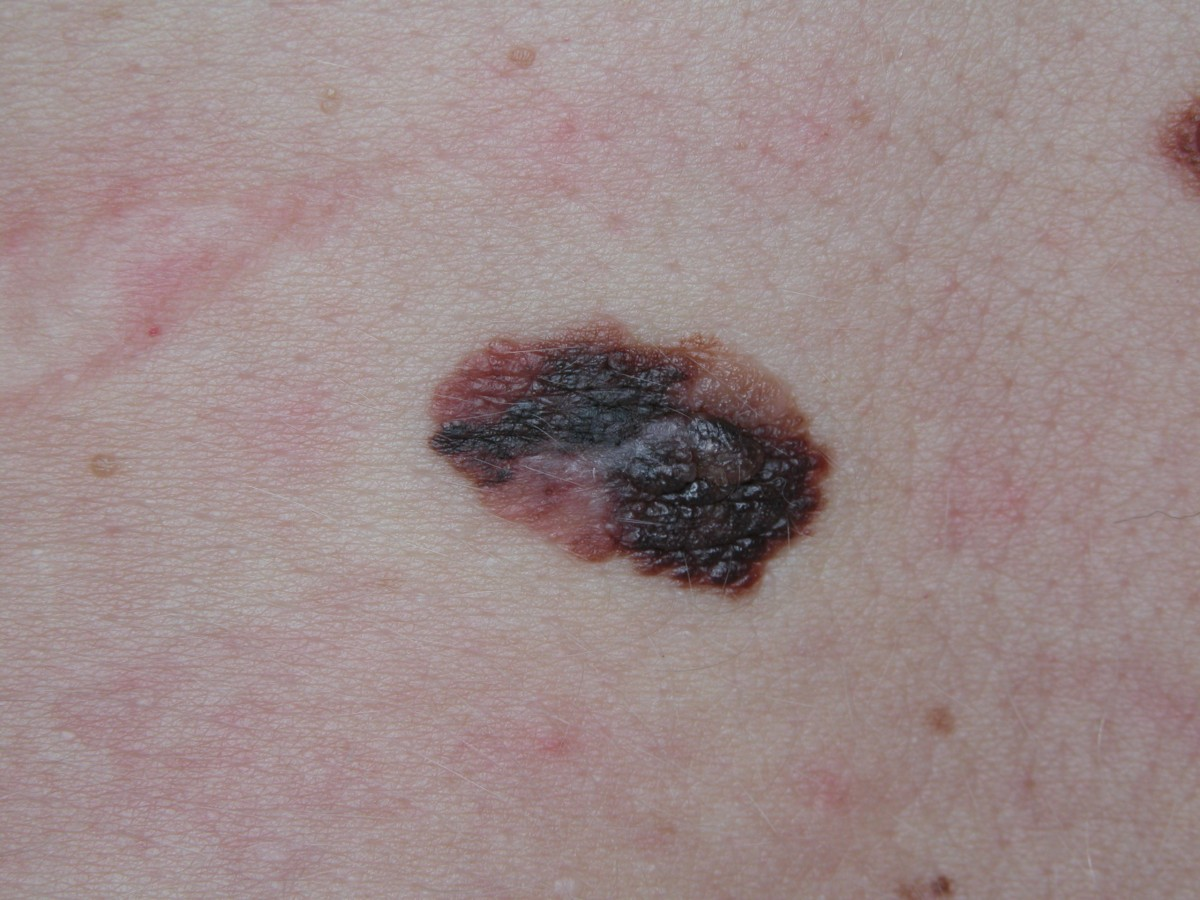
\includegraphics[scale=0.20]{fig/maligna-rana.png}
  \caption{Malígny melanóm. Zdroj \cite{Svehlik2012}}
  \label{fig:maligny-melanom}
\end{figure}

\subsection{Pooperačné rany}
Už ako samotný názov napovedá, ide o rany, ktoré vznikli v rámci operačného výkonu. Spôsob a vzhľad obnovenia integrity kože nerušenej pri operačnom výkone záleží na chirurgovi, ktorý zákrok vykonával. O tom, akým spôsobom sa ale bude rana hojiť, a ako bude vypadať výsledná jazva, rozhoduje celá rada ďalších faktorov.

Príčinou komplikovaného hojenia operačnej rany je väčšinou infekcia. Kontaminácia rany mikroorganizmami môže byť spôsobená samotným charakterom operácie, avšak ale aj porušením aseptických pravidiel, alebo následným preväzom. Väčšina ranných infekcií je avšak spôsobená mikroorganizmami, ktoré boli v organizme prítomné už pred vznikom infekcie. K najčastejším pôvodcom patria stafylokoky, streptokoky, klebsiely, kvasiny, alebo pseudomonády.

Prejavom takýchto rán je v rannom štádiu opuch a začervenanie rany a jej okolia. Ide o prejav zápalu, ktorým sa organizmus bráni pred poškodením. Tieto prejavy sú v rôznej miere zastúpené pri všetkých operačných ranách. Až prítomnosť hnisu je známkou infekcie. Infekcia sa prajavuje tak, že žltá, alebo nazelenalá tekutina sa hromadí v rane a zväčšuje jej objem, alebo dokonca vyteká. Rana sa potom následne rozpadá, jej stehy sú povlečené a priľahlé rany nekrotické. Infekcia zasahuje do rôznej hĺbky. V niektorých prípadoch sa obmedzuje iba na kožu a podkožie, v iných zase postihuje všetky vrstvy rany.
\begin{figure}[h]
  \centering
  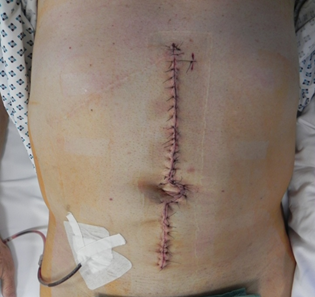
\includegraphics[scale=1]{fig/pooperacna-rana.png}
  \caption{Operačná rana po klasickej laparotómii. Zdroj \cite{XUKYT8x1LmEzzkqO}}
  \label{fig:pooperacna-rana}
\end{figure}

\section{Hojenie rán}
Hojenie je proces obnovovania tkaniva. Ide o jeden zo základných dejov, podieľajúci sa na prežití organizmu. Hojenie rany ovplyvňuje niekoľǩo faktorov, ktoré sa dajú rozdeliť na lokálne a celkové. Medzi lokálne faktory patrí porucha krvného zásobovania, stav okolitého tkaniva, pôsobenie tlaku, prítomnosť infekcie, nevhodné šicie materiály a technika, pohyb v rane, teplota, pH, dehydratácia a opuch. Medzi celkové faktory ovplyvňujúce hojenie patrí vek, celkový zdravotný stav pacienta, stav imunitného systému, anémia, strata krvi, podvýživa, nedostatok bielkovín, vplyv liekov, imobilita a psychický stav.

Hojenie rán prebieha v niekoľkých na seba nadväzujúcih fází a prebieha odlišne pri akútnych ranách a chronických ranách. Hojenie pri akútnych ranách prebieha v 3 hlavných fázach (ich zoznam je tu uvedený pre úplnosť, ich popis nie je v tomto kontexte dôležitý):
\begin{enumerate}
\item exsudatívna fáza
\item preliferačná fáza
\item diferenciačná fáza
\end{enumerate}
Hojenie chronických rán je o niečo komplikovanejšie. Tieto rany sa zaceľujú výstavbou nového tkaniva. Doba ich hojenia je veľmi zdĺhavá a závisí na rozsahu poškodenia tkaniva. Hojenie prebieha znovu v 3 hlavných fázach:
\begin{enumerate}
\item \textbf{fáza čistenia -} je potrebné zaistiť odlúčenie poškodených a odumretých tkanív. Liečba je zameraná na podporu samo-čistiacich procesov v kombinácií spolu s chirurgickým ošetrením.
\item \textbf{fáza granulácie -} po vyčistení z fáze 1 sú vytvorené podmienky pre rast a delenie nových buniek a vzniká granulačné tkanivo.
\item \textbf{fáza epitelizácie -} dochádza k deleniu a pohybu kožných buniek. Z okrajov rany prerastá epitel a pokrýva granulačné tkanivo novo-vytvorenou kožou.
\end{enumerate}

Hodnotenie hojenia rany prebieha podľa niekoľkých základných vlastností. Medzi tieto vlastnosti patrí príčina vzniku, vek rany, veľkosť, okraje, lokalizácia, hĺbka, vzhľad spodiny, bolestivosť, prítomnosť infekcie, množstvo sekrécie, zápach, okolie rany a súčasná a minulá lokálna terapia.